\section{Two-level Fingerprinting technique}\label{sec:two-level-fp}
Guo et al. \cite{guo2006fingerprinting} propose a fingerprinting technique for protecting numerical relational data from illegal duplication and redistribution. 
The fingerprint embedding scheme contains two embedding processes. 
In the first embedding process, a unique fingerprint that identifies a specific buyer is embedded in relational data using a secret key known only to the owner of the database.
The fingerprint can be detected using the same secret key to prove ownership at a numerical confidence level. 
The second embedding process is designed for verifying the extracted fingerprint. 
Thus, the scheme provides ownership identification and illegal distributor identification on two separate numerical confidence levels. 

The scheme uses the primary key for the identification of each tuple and for embedding the fingerprint. 
The proposed technique is marking a single attribute that is predefined based on practical attribute properties, taking into account that the embedding algorithm introduces small distortions to the least significant bits of the values. 
The scheme-specific notation is shown in \Cref{tab:two-level-fingerprint-notation}. For the rest of the notations we refer to \Cref{table:notation}.

\begin{table}[ht]
    \centering
    \caption{Notation in the Two-level Scheme}
    \label{tab:two-level-fingerprint-notation}
    \begin{tabular}{|c|l|}
        \hline
         $1/\gamma_1$ & Marked ratio in the first embedding process  \\
         \hline
         $1/\gamma_2$ & Marked ration in the second embedding process \\
         \hline
         $\alpha_1$ & Significance level of the ownership\\
         \hline
         $\alpha_2$ & Significance level of each fingerprint bit \\
         \hline
         $\alpha_3$ & Significance level of the fingerprint \\
         \hline
    \end{tabular}
\end{table}

\subsection{Algorithms}
\paragraph{Insertion} The insertion (embedding) algorithm whose, pseudocode is shown in \Cref{alg:two-level-insertion}, combines two embedding processes. 
The first process (lines 1-6) uses a cryptographic hash function to produce hash values of a concatenation of the secret key and primary key. The hash values are used to group tuples into $L$ groups. 
Each group is associated with one fingerprint bit $f_i$. 
Since the hash results are uniformly distributed, each group is expected to have a similar number of tuples. 
The fingerprint bit $f_i$ is part of a seed for a hash function that decides which tuples in the group $i$ will be marked by $f_i$. 
We concatenate the fingerprint bit $f_i$, primary key $r.P$ and secret key $\mathcal{K}$, use it as a seed for the hash function and compute the modulo by $\gamma_1$. 
Due to the uniformity of a hash function, on average $\frac{1}{\gamma_1}$ is the fraction of tuples that will be selected for marking. 
A different seed, created by the same values permuted, is then used in a hash function that decides which LSB will be marked by $f_i$ in the marking process. 
The described marking pattern is used to verify the ownership independently from the fingerprint. 

The second embedding process (lines 7-17) for marking considers only the tuples that have not already been marked in the first embedding process to avoid overlapping. 
This process uses the fingerprint itself as a secret key. 
Similarly to the first process, the hash function results are used to select the tuples and LSBs to be marked. 
The selected bit is marked "0" if the hash result of secret key $\mathcal{K}$ concatenated with primary key $r.P$ is odd, otherwise "1". 
The granularity of the second embedding process is controlled by $\gamma_2$.
The fraction of tuples marked in the second process is $(1-\frac{1}{\gamma_1})*\frac{1}{\gamma_2}$.
Thus, the total fraction of tuples marked can be calculated as in \Cref{eq:total-gamma}.
\begin{equation}\label{eq:total-gamma}
    \frac{1}{\gamma}=\frac{1}{\gamma_1}+(1-\frac{1}{\gamma_1})*\frac{1}{\gamma_2}
\end{equation}

\begin{algorithm}
    \KwIn{dataset $\mathcal{R}$ with primary key $P$, buyer's fingerprint $\mathcal{F}$}
    \ForEach{tuple $r \in \mathcal{R}$}
    {
        $i = \mathcal{H}(r.P|\mathcal{K})$ mod $L$ \\
        group[$i$] $\leftarrow r$ \\ 
        \uIf{$\mathcal{H}(f_i|r.P|\mathcal{K}$) mod $\gamma_1 == 0$}{
            $j = \mathcal{H}(r.P|\mathcal{K}|f_i)$ mod $\xi$\\
            $LSB(j,r)=f_i$ \\
        }
        \uElseIf{$\mathcal{H}(\mathcal{F}|r.P|\mathcal{K})$ mod $\gamma_2==0$}
        {
            $j=\mathcal{H}(r.P|\mathcal{K}|\mathcal{F})$ mod $\xi$\\
            \If{$\mathcal{H}(\mathcal{K}|r.P)$ mod 2 == 0}
            {
                $LSB(r,j)=0$\\
            }
            \Else{
                $LSB(r,j)=0$\\
            }
        }
        \uElse{}{
            do nothing to this tuple\\
        }
        
    }
  \KwOut{fingerprinted dataset $\mathcal{R}'$}
  \caption{Two-level Scheme: Insertion Algorithm}
  \label{alg:two-level-insertion} 
\end{algorithm}

\paragraph{Detection}
The fingerprint detection (fingerprint extraction) algorithm consists of three tasks: 
\begin{enumerate}
    \item Ownership verification
    \item Fingerprint extraction
    \item Fingerprint verification
\end{enumerate}
The first task is to find the pattern to verify the ownership, the second is to extract the suspect's fingerprint and finally, the third task is verifying the extracted fingerprint. \Cref{alg:two-level-extraction} comprise the first two tasks - ownership verification and fingerprint extraction. 
Fingerprint verification is described by \Cref{alg:two-level-verification}.
All parameters and the secret key should be the same as used in the embedding algorithm. 

\begin{algorithm}
    \KwIn{suspect relation $\mathcal{R}'$ with primary key $P'$}
    total\_count$_0$, total\_count$_1$, match\_count$_0$, match\_count$_1$ = \textit{detect}($\mathcal{R}'$)\\
    total\_count = total\_count$_0$ + total\_count$_1$\\
    match\_count = match\_count$_0$ + match\_count$_1$\\
    \If{match\_count > \textit{threshold(total\_count, $\alpha_1$)}}
    {
        \ForEach{tuple $r \in \mathcal{R}$}
        {
            $i = \mathcal{H}(r.P|\mathcal{K})$ mod $L$ \\
            group[$i$] $\leftarrow r$ \\ 
        }
        \ForEach{group[i]}
        {
            total\_count$_0$, total\_count$_1$, match\_count$_0$, match\_count$_1$ = \textit{detect}(group[i])\\
            \uIf{match\_count$_0$>threshold(total\_count$_0$,$\alpha_2$)}
            {
                $f_i$ = 0 \\
            }
            \uElseIf{match\_count$_1$>threshold(total\_count$_1$,$\alpha_2$)}
            {
                $f_i = 1$ \\
            }
            \Else{fail to extract $f_i$}
        }
    }
    \Return{fingerprint $\mathcal{F}$}
    \caption{Two-level Scheme: Fingerprint Extraction Algorithm}
    \label{alg:two-level-extraction}
\end{algorithm}

\begin{algorithm}
    \textit{detect}(relation $\mathcal{R}$):\\
    total\_count$_0$ = total\_count$_1$ = match\_count$_0$ = match\_count$_1$ = 0 \\
    \ForEach{tuple $r \in \mathcal{R}$}
    {
        \If{$\mathcal{H}(1|r.P|\mathcal{K})$ mod $\gamma_1 == 0$} 
        {
            // $subset_1$ \\
            total\_count$_1$++\\
            $j=\mathcal{H}(r.P|\mathcal{K}|1)$ mod $\xi$\\
            \If{$j^{th}$ bit is 1}
            {
                match\_count$_1$++\\
            }
        }
        \If{$\mathcal{H}(0|r.P|\mathcal{K})$ mod $\gamma_1 == 0$} 
        {
            // $subset_0$ \\
            total\_count$_0$++\\
            $j=\mathcal{H}(r.P|\mathcal{K}|0)$ mod $\xi$\\
            \If{$j^{th}$ bit is 0}
            {
                match\_count$_0$++\\
            }
        }
    }
    \Return{total\_count$_0$, total\_count$_1$, match\_count$_0$, match\_count$_1$}
    \caption{Two-level Scheme: Subroutine \textit{detect}}
    \label{alg:subroutine-detect-two-level}
\end{algorithm}


\begin{algorithm}
    \textit{threshold}(n, $\alpha$):\\
    \Return{minimum integer $m$ that satisfies $\sum_{k=m}^{n}{c^k_n}(\frac{1}{2})^n < \alpha$}
    \caption{Two-level Scheme: Subroutine \textit{threshold}}
    \label{alg:subroutine-threshold}
\end{algorithm}

The first step of the extraction algorithm is ownership verification. 
We use the original secret key $\mathcal{K}$ to find the pattern embedded in the embedding process. 
Firstly, we use subroutine \textit{detect} (\Cref{alg:subroutine-detect-two-level}) to identify the candidate set of tuples for detecting marks. 
The candidate tuples are sorted into $subset_0$ and $subset_1$ depending on the conditions in lines 4 and 12 of the subroutine \textit{detect}. 
If a tuple satisfies both conditions, it is included in both $subset_0$ and $subset_1$. 
$total\_count_0$ and $total\_count_1$ count the number of candidate tuples in $subset_0$ and $subset_1$, respectively. 
These steps ensure that all of the tuples selected for marking in the embedding process (\Cref{alg:two-level-insertion}, line 4) are going to be selected as candidate tuples (although the inverse does not hold; there exist candidate tuples that were not chosen for marking in the first embedding process). The total number of candidate tuples $total\_count=total\_count_0+total\_count_1$ will be $\approx\eta/\gamma_1 + \eta/\gamma_1=2\eta/\gamma_1$.

Once the tuple is selected as a candidate, the algorithm checks whether the bit positions that were supposed to be marked in the embedding process in the candidate tuples are the correct values. 
In line 7 we calculate the same hash as in embedding process - $\mathcal{H}(r.P|\mathcal{K}|1)$ to obtain the bit position that should contain a mark, and in lines 8-10 we record if the mark is correct by the count variable $match\_count_1$. 
The same steps are done for candidate tuples from $subset_0$ in lines 15-18. 
The total number of matches from the candidate tuples is then $match\_count=match\_count_0+match\_count_1$. 
Note that in unaffected fingerprinted data, we expect to see $\eta/\gamma_1$ matches that correspond to tuples marked in the fist embedding process. 
This algorithm further produces more "fake" matches, about $\eta/2\gamma_1$ of them, so in total the rough expectation is $match\_count = 3\eta/2\gamma_1$.

From this extraction phase, the ratio of matches and the total number of candidate tuples is $match\_count/total\_count=75\%$. 
This forms a special pattern, and a probability to detect such a pattern in unmarked data is rather small.
The authors propose a threshold value which satisfies:
\begin{equation}
    P\{MATCH\_COUNT > threshold | total\_count\} < \alpha
\end{equation}
i.e. the probability to find matches more than the threshold is less than $alpha$ in a non-marked relation, where $alpha\in(0,1)$ is a small value called significance level. 
Thus, once such a pattern is detected, we can claim that the relation must have been modified by our insertion algorithm at the confidence level of $(1-\alpha)$.
The threshold (\Cref{alg:subroutine-threshold}) for a given $total\_count$ is calculated as \Cref{eq:threshold}.

\textit{threshold = minimum integer m that satisfies}
\begin{equation}
\label{eq:threshold}
    \sum_{k=m}^{n}c_n^k\Big(\frac{1}{2}\Big)^n<\alpha \\
\end{equation}
\textit{where}
\begin{equation}
    c_n^k=\frac{n!}{k!(n-k)!} ; n=total\_count
\end{equation}
In line 4 of \Cref{alg:two-level-extraction} we compare the total number of matches with the threshold. 
If the number of matches is larger than the threshold, the ownership verification succeeded; otherwise, the ownership cannot be claimed.

When the ownership verification is done, the algorithm attempts to extract the fingerprint to track the buyer that leaked the data without the authorisation.
The procedure starts with line 5 of \Cref{alg:two-level-extraction} and like the insertion algorithm forms the same $L$ groups. 
The group represents the subset of tuples that are marked with the same fingerprint $f_i$.
Therefore, for each group the candidate tuples and matches are calculated using again the subroutine \textit{detect} (\Cref{alg:detect-subroutine}) to extract the value of each fingerprint bit. 
For this phase, we use a significance level $\alpha_2$. 
A fingerprint bit $f_i$ is claimed to be 0 at confidence level $(1-\alpha_2)$ if the $match\_count_0$ is larger than the threshold calculated with the number of candidate tuples from the group that might contain mark $0$ from the embedding phase - $total\_count_0$ and $\alpha_2$. 
Following the analogy, fingerprint bit $f_i$ is claimed to be 1 if the $match\_count_1$ is larger than the corresponding threshold.
If neither $match\_count_0$ nor $match\_count_1$ exceed the corresponding threshold, the fingerprint bit value cannot be decided. 
The output of \Cref{alg:two-level-extraction} is an extracted candidate fingerprint which needs further verification. 

\begin{algorithm}
    \KwIn{suspect relation $\mathcal{R}'$, suspect fingerprint $\mathcal{F}'$}
    \ForEach{tuple $r \in \mathcal{R}'$}
    {
        \If{$\mathcal{H}(\mathcal{F}'|r.P|\mathcal{K})$ mod $\gamma_2$==0 $\&\&$ $\mathcal{H}(f'_i)|r.P|\mathcal{K}$ mod $\gamma_1$!=0}
        {
        total\_count++\\
        $j=\mathcal{H}(r.P|\mathcal{K}|\mathcal{F}')$ mod $\xi$\\
        \uIf{$\mathcal{H}(\mathcal{K}|r.P)$ is even $\&\&$ $j^{th}$ bit is 0}
        {
            match\_count++\\
        }
        \uElseIf{$\mathcal{H}(\mathcal{K}|r.P)$ is odd $\&\&$ $j^{th}$ bit is 1}
        {
        match\_count++\\
        }
        }
    }
    \If{match\_count>\textit{threshold}(total\_count, $\alpha_3$)}
    {
        \KwOut{the fingerprint is verified}
    }
    \Else{
        \KwOut{the fingerprint is not verified}
    }
    \caption{Two-level Scheme: Fingerprint Verification Algorithm}
    \label{alg:two-level-verification}
\end{algorithm}

Using the \Cref{alg:two-level-verification}, we identify the exact fingerprint from the candidate set of suspect fingerprints produced by \Cref{alg:two-level-extraction}. 
In this phase, we detect the embedding pattern from the second phase of fingerprint embedding algorithm at a confidence level of $(1-\alpha_3)$.
Following the steps of the second phase of the fingerprint insertion algorithm, we consider only the tuples that have not been marked in the first embedding process. 
The pattern is detected using the owner's secret key $\mathcal{K}$ and the candidate fingerprint $\mathcal{F}$.
The \Cref{alg:two-level-verification} in line 3 counts the candidate tuples that are supposed to be marked, and depending on the hash value and value of the corresponding fingerprint bit, counts the matches in lines 6 or 8, depending on whether the bit value is $0$ or $1$. 
Note that in this phase if the data is unaffected, the parameters and the secret key are the same as in the insertion algorithm, and also the correct fingerprint is extracted in the previous phase, then the number of candidate tuples $total\_count$ and number of matches $match\_count$ is expected to be equal.
The number of matches is once again compared to the threshold calculated from $total\_count$ and significance level $\alpha_3$. 
If the number of matches satisfies the condition in line 11, we may claim that the fingerprint $\mathcal{F}$ is verified at confidence level $(1-\alpha_3)$.

\subsection{Properties and discussion}
We mentioned in the previous section that the extraction algorithm relies on finding a certain number of matches that would confirm the mark pattern is embedded in the data.
The confidence levels of the fingerprint extraction process (i.e. the converse process to the first embedding processes) are defined by significance level parameters $\alpha_1$ and $\alpha_2$ that are used to calculate the $threshold$ value. 
To achieve a high confidence level of ownership, e.g. 99\% ($\alpha_1 = 0.01$), the condition in line 4 of \Cref{alg:two-level-extraction} has to be satisfied.

\begin{figure}
    \centering
    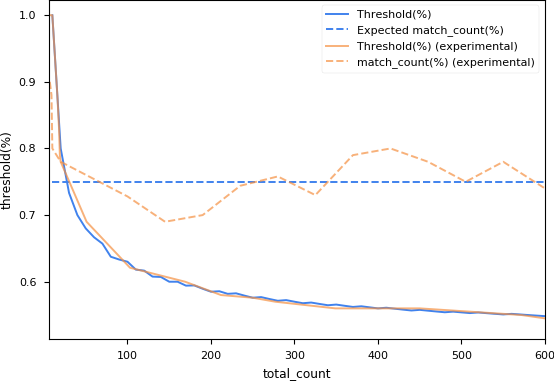
\includegraphics[width=\textwidth]{Figures/threshold_two-level.png}
    \caption{Portion of match\_count and \textit{threshold} for different total\_count to achieve the ownership confidence level 99\% ($\alpha_1=0.01$)}
    \label{fig:threshold-ownership}
\end{figure}

\Cref{fig:threshold-ownership} shows, for a fixed $\alpha_1=0.01$, the thresholds for different values of $total\_count$ as a fraction of $total\_count$ (continuous blue line).
The dashed blue line is the expected fraction of $match\_count$ out of $total\_count$ (75\%).
We can see that for the $total\_count$ larger than $\approx 30$ the previously mentioned condition is satisfied and the extraction algorithm can verify the ownership with a confidence level of 99\%. 
The statement is confirmed with the experimental results shown by the orange lines in the figure.
The experiments are run on Forest Cover Type data with fingerprint length $L=96$.
The $match\_count$ value in the experiments is $75\%(total\_count)\pm5\%$, according to the expectation. Furthermore, the lower limit for $total\_count$ to have 99\% confidence level for ownership is shown to be around 30. 
Therefore, \Cref{eq:ownership-verification} needs to be satisfied for the correct ownership verification.

\begin{equation}\label{eq:ownership-verification}
    2\eta/\gamma_1 > 30 (\alpha_1=0.01)
\end{equation}

For the real-life datasets with hundreds or thousands of tuples this is rather easy to achieve (e.g. for Forest Cover Type data, setting $\gamma_1=200$ results in $total\_count \approx 5,800$).

The second phase of detection algorithm - the fingerprint extraction - identifies each bit individually from the associated group of tuples. 
The process of comparing the matching bits to the threshold value is in this phase controlled by $\alpha_2$.
If the number of matches of a single bit value is larger than the threshold, the bit is decided to be that value (conditions in lines 11 and 13 of \Cref{alg:two-level-extraction}).

\begin{figure}
\centering
    \subfloat[$\alpha_2=0.01$]{{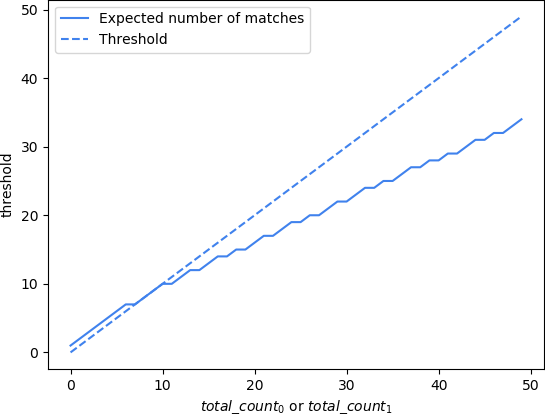
\includegraphics[width=6.7cm]{Figures/fingerprint-extraction-threshold-scrnsh.png} }}
    \qquad
    \subfloat[$\alpha_2=0.1$]{{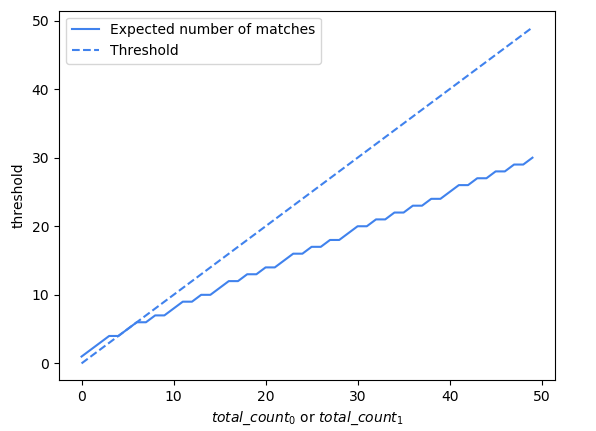
\includegraphics[width=6.7cm]{Figures/fingerprint-extraction-threshold-90.png} }}
    \caption{Threshold in subsets of unaffected marked data for different $total\_count_i$ to achieve confidence level of each bit of 99\% (a) and 90\% (b)}
    \label{fig:threshold-fingerprint-extraction}
\end{figure}

\Cref{fig:threshold-fingerprint-extraction} shows threshold values in a subset, depending on the total number of tuples in a subset. 
A dashed line represents the expected number of matches in a marked group of unaffected fingerprinted data.
We show the relation between thresholds and the number of matches for different levels of confidence - 99\% and 90\%.
Generally, the more tuples are selected into a subset, the more robust the fingerprint is. 
For reaching the confidence level of 99\%, $total\_count_i$  must be at least 8 for a trusted pattern to be found, while for 90\% confidence that lower limit is 4. 
Therefore, \Cref{eq:extraction-99} must be satisfied to obtain the successful marking pattern with confidence 99\% and \Cref{eq:extraction-90} with confidence 90\%.

\begin{equation}\label{eq:extraction-99}
    \eta/(\gamma_1 * L) > 7 (\alpha_2=0.01)
\end{equation}

\begin{equation}\label{eq:extraction-90}
    \eta/(\gamma_1 * L) > 3 (\alpha_2=0.1)
\end{equation}

In the real implementation $\eta/(\gamma_1 * L)$ should be rather larger than suggested in \Cref{eq:extraction-99,eq:extraction-90} because of the deviation introduced by random distribution of tuples into $L$ groups. 

\paragraph{}
The proposed technique has a limitation that it embeds the fingerprint in only one, initially chosen attribute. 
However, this approach is vulnerable to a vertical attack (attribute deletion attack) where the attacker can delete the fingerprint by removing the entire attribute. 
To avoid the possibility of such attack in multi-attribute datasets and for further experiments with this scheme, we slightly redesign the embedding and extraction process such that all attributes appear as candidates for marking. 
The simple modification is the reinterpretation of the term $LSB(r,j)$ in \Cref{alg:two-level-insertion}.
In this notation $LSB(r,j)$ represents the $j-th$ bit from the set of least significant bits available for marking of \textit{all} attribute values from the tuple $r$ (instead of only one predefined attribute).
Pseudo-randomness of this step ensures uniformly distributed marks over all attributes. 

